\documentclass[12pt]{scrartcl}

 

\usepackage[utf8]{inputenc}

\usepackage[T1]{fontenc}

\usepackage{lmodern}

\usepackage[ngerman]{babel}

\usepackage{amsmath}

\usepackage{graphicx}


 

\title{Versuch AK1\\ Ultraschall}

\author{Frederik Strothmann, Henrik Jürgens}

\date{\today}


\begin{document}


 %deckblatt erstellen

\maketitle
\tableofcontents
\newpage

%einleitung zu dem experiment

\section{Einleitung}
Mit einem System aus piezoelektrischen Ultraschallsendern und -empfängern wird die Schallgeschwindigkeit in Luft
bestimmt nach der Phasen- und der Laufzeitmethode. Bei Kenntnis der Schallgeschwindigkeit kann die Laufzeitmethode zur Entfernungsmessung eingesetzt werden (Echolotprinzip). Eine Anordnung mit zwei gleichen Ultraschallsendern wirkt wie ein Doppelspalt und liefert ein typisches
Ultraschall-Interferenzmuster, das ausgemessen werden soll.
Außerdem sollen noch die elektrischen Eigenschaften des Piezosenders (Impedanz) untersucht werden.

%versuchsaufbau mit skizze

\section{Versuchsaufbau}


\section{Versuchsdurchführung}


\subsection{Praktische Durchführung}

\subsubsection{Impedanzmessung}
\begin{itemize}
\item[(a)]
Um die elektrischen Eigenschaften eines Barium-Titanat-Ultraschallgenerators zu untersuchen, wird eine Schaltung gemäß Abb. \ref{fig:impedanz}
aufgebaut. Stellen Sie am Funktionsgenerator ein Sinussignal mit einer Amplitude von etwa 5 V ein.
%bitte Abb.7 aus der Versuchsanleitung einfügen, welche grade referenziert werden sollte "Aufbau zur Impedanzmessung"
\begin{figure}[htbp] 
  \centering
    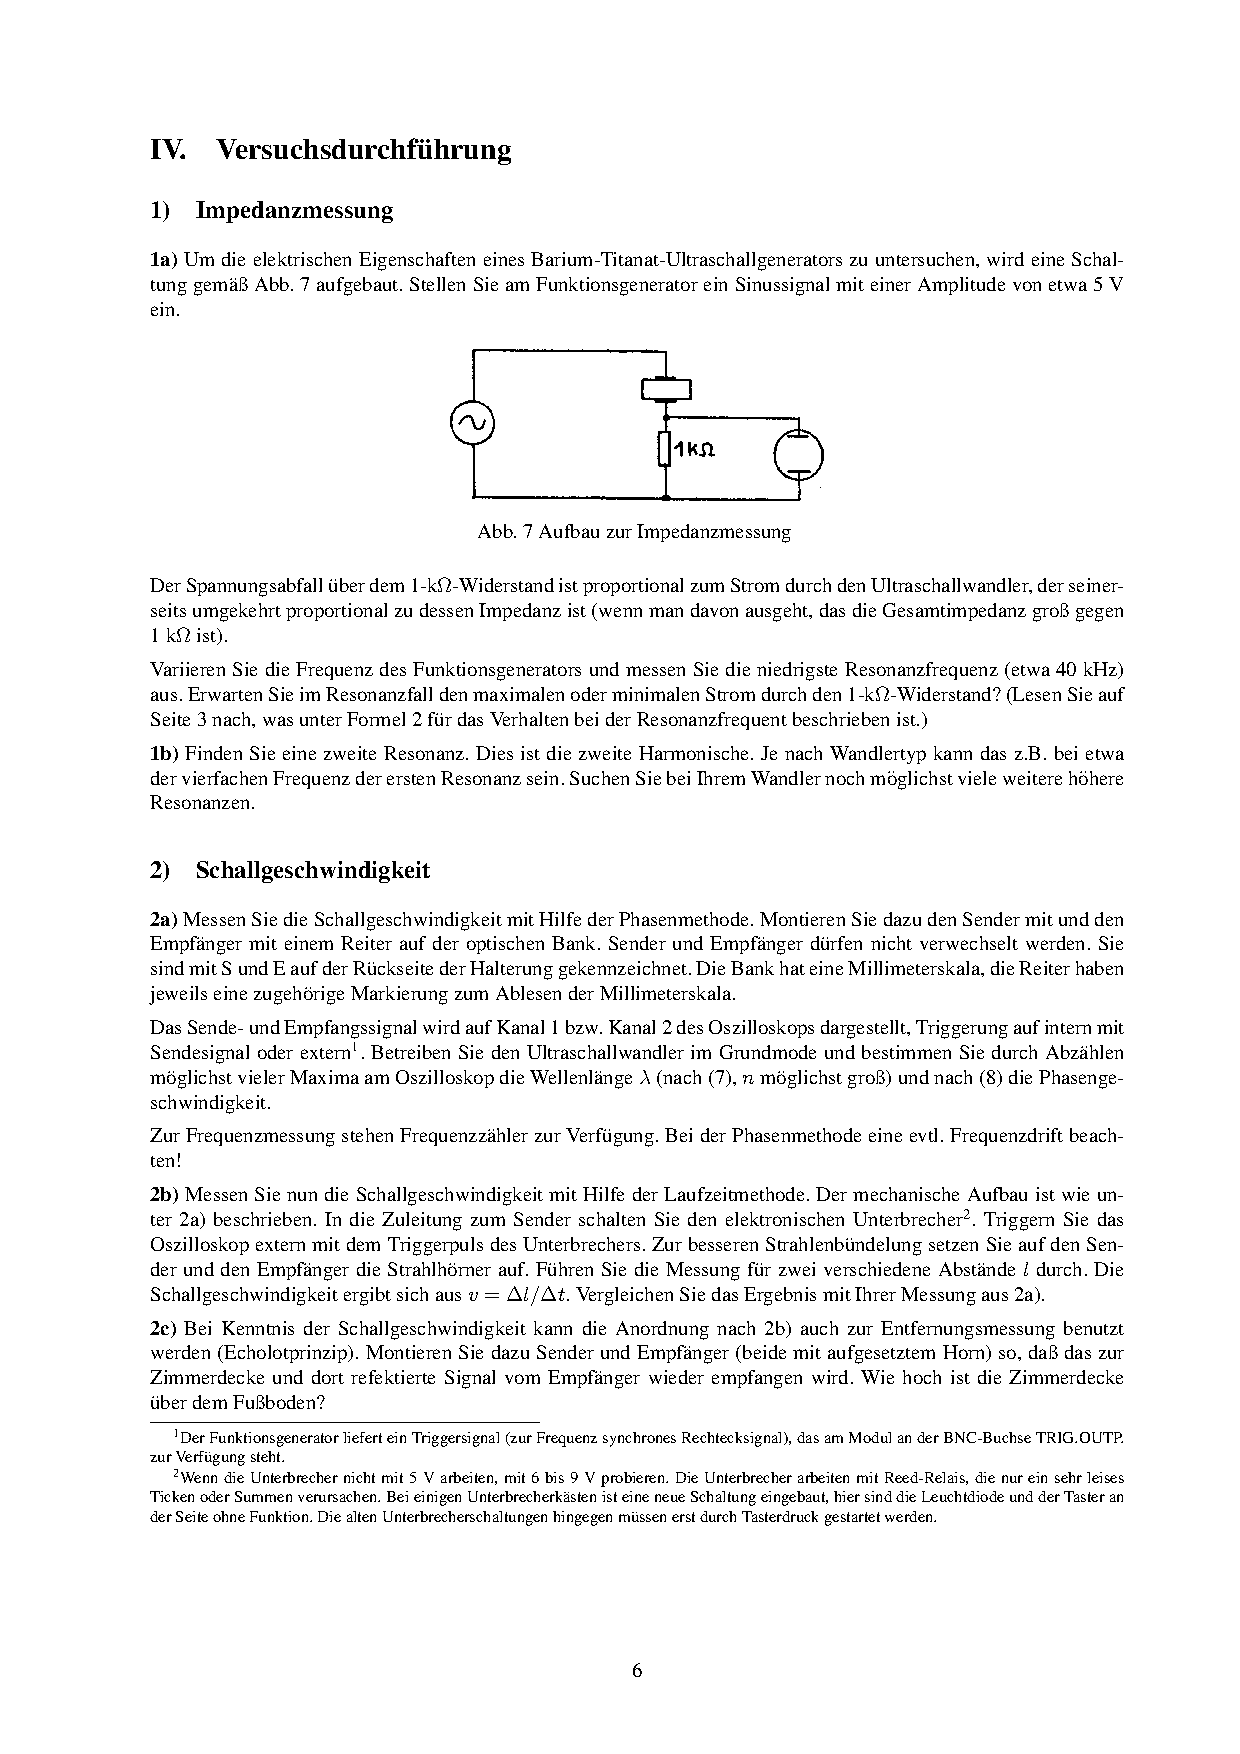
\includegraphics[trim = 20mm 210mm 20mm 55mm, clip, scale = 1]{impedanz.pdf}
  	\caption[Schaltskizze des Versuchsaufbaus]{Schaltskizze des Versuchsaufbaus\footnotemark}
  \label{fig:impedanz}
\end{figure}
\footnotetext{Abbildung entnommen von http://www.atlas.uni-wuppertal.de/~kind/AK1.pdf Seite 6 am 30.08.2014}
Der Spannungsabfall über dem 1-k$\Omega$-Widerstand ist proportional zum Strom durch den Ultraschallwandler, der seinerseits umgekehrt proportional zu dessen Impedanz ist (wenn man davon ausgeht, das die Gesamtimpedanz groß gegen 1 k$\Omega$ ist).
Variieren Sie die Frequenz des Funktionsgenerators und messen Sie die niedrigste Resonanzfrequenz (etwa 40 kHz)
aus. Erwarten Sie im Resonanzfall den maximalen oder minimalen Strom durch den 1-k$\Omega$-Widerstand? 
%(Lesen Sie auf Seite 3 nach, was unter Formel 2 für das Verhalten bei der Resonanzfrequenz beschrieben ist.)
\item[(b)]
Finden Sie eine zweite Resonanz. Dies ist die zweite Harmonische. Je nach Wandlertyp kann das z.B. bei etwa der vierfachen Frequenz der ersten Resonanz sein. Suchen Sie bei Ihrem Wandler noch möglichst viele weitere höhere
Resonanzen.
\end{itemize}
\subsubsection{Schallgeschwindigkeit}
\begin{itemize}
\item[(a)]
Messen Sie die Schallgeschwindigkeit mit Hilfe der Phasenmethode. Montieren Sie dazu den Sender mit und den Empfänger mit einem Reiter auf der optischen Bank. Sender und Empfänger dürfen nicht verwechselt werden. Sie sind mit S und E auf der Rückseite der Halterung gekennzeichnet. Die Bank hat eine Millimeterskala, die Reiter haben
jeweils eine zugehörige Markierung zum Ablesen der Millimeterskala. Das Sende- und Empfangssignal wird auf Kanal 1 bzw. Kanal 2 des Oszilloskops dargestellt, Triggerung auf intern mit Sendesignal oder extern
\footnote{Der Funktionsgenerator liefert ein Triggersignal (zur Frequenz synchrones Rechtecksignal), das am Modul an der BNC-Buchse TRIG.OUTP. zur Verfügung steht.}. Betreiben Sie den Ultraschallwandler im Grundmode und bestimmen Sie durch Abzählen möglichst vieler Maxima am Oszilloskop die Wellenlänge $\lambda$
%(nach Formel \ref{}, n möglichst groß) 
und nach Formel
%\ref{}
die Phasengeschwindigkeit.
Zur Frequenzmessung stehen Frequenzzähler zur Verfügung. Bei der Phasenmethode einen evtl. Frequenzdrift beachten!
\item[(b)]
Messen Sie nun die Schallgeschwindigkeit mit Hilfe der Laufzeitmethode. Der mechanische Aufbau ist wie unter (a) beschrieben. In die Zuleitung zum Sender schalten Sie den elektronischen Unterbrecher \footnote{Wenn die Unterbrecher nicht mit 5 V arbeiten, mit 6 bis 9 V probieren. Die Unterbrecher arbeiten mit Reed-Relais, die nur ein sehr leises Ticken oder Summen verursachen. Bei einigen Unterbrecherkästen ist eine neue Schaltung eingebaut, hier sind die Leuchtdiode und der Taster an der Seite ohne Funktion. Die alten Unterbrecherschaltungen hingegen müssen erst durch Tasterdruck gestartet werden.}. Triggern Sie das Oszilloskop extern mit dem Triggerpuls des Unterbrechers. Zur besseren Strahlenbündelung setzen Sie auf den Sender und den Empfänger die Strahlhörner auf. Führen Sie die Messung für zwei verschiedene Abstände
l durch. Die Schallgeschwindigkeit ergibt sich aus $v = \frac{\Delta l}{\Delta t}$. Vergleichen Sie das Ergebnis mit Ihrer Messung aus (a).
\item[(c)]
Bei Kenntnis der Schallgeschwindigkeit kann die Anordnung nach (b) auch zur Entfernungsmessung benutzt werden (Echolotprinzip). Montieren Sie dazu Sender und Empfänger (beide mit aufgesetztem Horn) so, daß das zur Zimmerdecke und dort refektierte Signal vom Empfänger wieder empfangen wird. Wie hoch ist die Zimmerdecke über dem Fußboden?
\end{itemize}
\subsubsection{Interferenz am Doppelspalt}
\begin{itemize}
\item[(a)]
Messen Sie das Beugungbild eines Doppelspaltes. Aus aufbautechnischen Gründen wird hierbei der Doppelsender um seine Symmetrieachse gedreht und der Empfänger fest am Ort belassen. Der Doppelsender ist auf einem Drehtisch montiert. (Zubehör zur optischen Bank). Den Empfänger montieren Sie
in ca. 1 m Abstand auf einen festen Reiter (achten Sie auf gleiche Höhe zwischen Sender und Empfänger). Da die Transducer des Doppelsenders aus einer anderen Bauserie stammen können als die Einzelsender, müssen Sie die Betriebsfrequenz neu einstellen und am Oszilloskop erneut bestimmen bzw. am Frequenzzähler ablesen. Die optimale Frequenz steht evtl. auf der Platine mit dem Doppelsender. Sinnvoll ist, die Frequenz so zu wählen, daß die Minima des Interferenzmusters
besonders ausgeprägt sind. Überlegen Sie: Was muß für die Amplituden der beiden Sender gelten? Sie können sich die Einzelamplituden am Oszilloskop ansehen, wenn Sie jeweils einen der beiden Sender mit dem Finger abdecken.
Messen Sie die Empfangamplitude für verschiedene Richtungswinkel des Doppelsenders zur Empfängerrichung (alle 2$^{\circ}$ im Bereich $\pm 50^{\circ}$). Tragen Sie die Empfangsamplitude gegen den Richtungswinkel auf. Bestimmen Sie aus dem Abstand des Minimums die Wellenlänge gemäß
\begin{align}
\frac{\lambda}{2} = l\sin(\Phi)
\end{align}
mit l: Abstand der Schallquellen.
Errechnen Sie hieraus mit Hilfe der vorher berechneten Schallgeschwindigkeit $c$ die Frequenz ($f = \frac{c}{\lambda}$) und vergleichen Sie diesen Wert mit dem Ihrer Messung mit dem Oszilloskop.
\end{itemize}
\subsection{Theoretische Durchführung}
\begin{enumerate}
\item[2.]
\begin{enumerate}
\item[(a)]
Die Formel für die Wellenlänge $\lambda$ ist:
\begin{align}
\lambda = \frac{\Delta l}{\Delta \Phi} 2\pi
= \frac{\Delta l}{n}
\end{align}
$n$ die Anzahl der überstrichenen "Wellenberge", $\Delta \Phi$ der Überstrichene Winkel.
\begin{align}
v_{\text{Ph}} = \lambda f
\end{align}
$v_{\text{Ph}}$ die Phasengeschwindigkeit des Schalls und $f$ die Frequenz des Sinusgenerators.
\item[(b)]
Die Formel für die Gruppengeschwindigkeit $v_{\text{Gr}}$ ist:
\begin{align}
v_{\text{Gr}} = \frac{l1-l2}{\Delta t1 - \Delta t2}
\end{align}
$l$ die Abstände zum Sender und $\Delta t$ die benötigte Zeit.
\item[(c)]
Die Formel für den Abstand ($d_{\text{Decke}}$) des Senders zur Decke ist:
\begin{align}
d_{\text{Decke}} = \frac{v \cdot \Delta t}{2}
\end{align}
$v$ die Schallgeschwindigkeit und $\Delta t$ die verstrichene Zeit.
\end{enumerate}

\item[3.]
\begin{align}
keineahnung
\end{align}

\end{enumerate}

\section{Messergebnisse}



\section{Auswertung}


\section{Diskussion}


 %Werte stimmen mit den Formeln überein/nicht überein

\end{document}

